\chapter{Sistemas de excitación. Control tensión-reactiva.}
	\section{Respuesta de sistemas.}
		\subsection{Sistemas de primer orden.}
			Sea el sistema con realimentación unitaria de la figura siguiente:
			\begin{figure}[H]
				\centering
					\begin{circuitikz}[scale=0.7]
						\tikzstyle{every node}=[font=\normalsize]
						\draw  (9.75,14) circle (0.5cm);
						\draw [->, >=Stealth] (7.75,14) -- (9.25,14)node[pos=0.25,above]{X(s)};
						\draw [->, >=Stealth] (10.25,14) -- (11.25,14);
						\draw  (11.25,14.75) rectangle  node {\normalsize G(s)} (13.5,13.25);
						\draw [short] (14.5,14) -- (14.5,12.5);
						\draw [short] (14.5,12.5) -- (9.75,12.5);
						\draw [->, >=Stealth] (9.75,12.5) -- (9.75,13.5);
						\node [font=\normalsize] at (9,14.25) {+};
						\node [font=\normalsize] at (10,13.25) {-};
						\node at (14.5,14) [circ] {};
						\draw [->, >=Stealth] (13.5,14) -- (15.5,14)node[pos=0.5,above]{Y(s)};
					\end{circuitikz}
			\end{figure}
			
			$G(s)$ se denomina "función de transferencia de la planta", y su comportamiento viene descrito por los polos y ceros que lo componen:
			\[G(s) = \dfrac{\prod ceros}{\prod polos} = \dfrac{b_0 + b_1 s + b_2 s^2\dots + b_m s^m}{a_0 + a_1 s + a_2 s^2\dots + a_n s^n}\]
			El sistema será estable si, en la función de transferencia global, el número de polos es mayor al de ceros: $n>m$.
			
			La función de transferencia del sistema es:
			\[M(s) = \dfrac{Y(s)}{X(s)} = \dfrac{G(s)}{1 + G(s)}\]
			
			
			Si una función $G(s)$ es de primer orden es de la forma:
			\[G(s) = \dfrac{K}{1+Ts} = \dfrac{\dfrac{K}{T}}{s+\dfrac{1}{T}}\]
			Donde $K$ es la ganancia del sistema (su valor cuando finaliza el transitorio) y $T$ la constante de tiempo del sistema.
			
			
			La respuesta a escalón de un sistema de primer orden es:
			\[y(t) = K\left(1-e^{-t/T}\right)\]
			
			
			Los sistemas de primer orden tienen un polo. Si el polo es positivo entonces el sistema es inestable, si es negativo es estable y si es 0 el sistema no converge y es críticamente estable:
			\begin{figure}[H]
				\begin{minipage}{0.5\textwidth}
					\begin{figure}[H]
						\centering
						\begin{circuitikz}
							\tikzstyle{every node}=[font=\normalsize]
							\draw [->, >=Stealth] (11.25,13) -- (15.5,13)node[pos=1,above]{Re};
							\draw [->, >=Stealth] (13.25,12.5) -- (13.25,15)node[pos=1,above]{Im};
							\node at (12.25,13) {$\times$};
							\draw [ color={rgb,255:red,0; green,128; blue,0}, ->, >=Stealth, dashed] (13,14.5) -- (11.25,14.5)node[pos=0.5,above]{Estable};
							\draw [ color={rgb,255:red,255; green,0; blue,0}, ->, >=Stealth, dashed] (13.5,14.5) -- (15.5,14.5)node[pos=0.5,above]{Inestable};
						\end{circuitikz}
						
						\label{fig:my_label}
					\end{figure}
				\end{minipage}
				\begin{minipage}{0.5\textwidth}
					\begin{figure}[H]
						\centering
						\begin{circuitikz}[scale = 0.8]
							\tikzstyle{every node}=[font=\normalsize]
							\draw [->, >=Stealth] (13.75,12.75) -- (17.5,12.75)node[pos=1,above]{t};
							\draw [->, >=Stealth] (14,12.5) -- (14,16)node[pos=1,right]{y};
							\draw [ color={rgb,255:red,0; green,128; blue,255}, short] (14,12.75) .. controls (14.25,14) and (14.25,15.5) .. (17.25,15.5);
							\draw [dashed] (17.25,15.5) -- (14,15.5)node[pos=1,left]{K};
						\end{circuitikz}
						
						\label{fig:my_label}
					\end{figure}
				\end{minipage}
			\end{figure}
			
			
			
			
		\subsection{Sistemas de segundo orden subamortiguados.}
			Sea el sistema con realimentación unitaria de la figura anterior. Si ahora $G(s)$ tiene 2 polos será de segundo orden. La posición de los polos de la función de transferencia del lazo abierto determina el lugar de las raíces, que muestra el comportamiento del sistema: si son complejos conjugados será subamortiguado.
			
			\begin{figure}[H]
				\begin{minipage}{0.5\textwidth}
					\[G(s) = \dfrac{K \omega_n^2}{s^2 + 2\xi \omega_n s + \omega_n^2}\]
					\[\sigma = \xi \omega_n \qquad \xi = \cos \theta\]
				\end{minipage}
				\begin{minipage}{0.5\textwidth}
					\begin{figure}[H]
						\centering
						\begin{circuitikz}
							\tikzstyle{every node}=[font=\normalsize]
							\draw [->, >=Stealth] (11.25,13) -- (14,13)node[pos=1,above]{Re};
							\draw [->, >=Stealth] (13.25,11) -- (13.25,15)node[pos=1,above]{Im};
							\node at (11.75,14.25) {$\times$};
							\node at (11.75,11.75) {$\times$};
							\draw [short] (13.25,13) -- (11.75,14.25)node[pos=0.5,above, sloped]{$\omega_n$};
							\draw [dashed] (11.75,14.25) -- (13.25,14.25)node[pos=1,right]{$j\omega_d$};
							\draw [dashed] (11.75,14.25) -- (11.75,11.75)node[pos=0.4,left]{$\sigma$};
							\draw [short] (11.75,11.75) -- (13.25,13);
							\draw [<->, >=Stealth] (12.5,13.6) .. controls (12.25,13.3) and (12.25,13.25) .. (12.25,13)node[pos=0.5,left]{$\theta$};
							\draw [ color={rgb,255:red,0; green,128; blue,255}, short] (11.75,11.75) -- (11.75,11);
							\draw [ color={rgb,255:red,0; green,128; blue,255}, short] (11.75,14.25) -- (11.75,15);
						\end{circuitikz}
						
						\label{fig:my_label}
					\end{figure}
				\end{minipage}
			\end{figure}
			
			Respuesta a escalón en sistemas subamortiguados ($0 <\xi < 0.707$):
			\[y(t) = K\left(1-\dfrac{e^{-\sigma t}}{\sqrt{1-\xi^2}} \sin (\omega_d t + \theta)\right)\]
			
			\begin{figure}[H]
				\begin{minipage}{0.5\textwidth}
					\begin{itemize}
						\item \textbf{\textit{Tiempo de establecimiento:}} tiempo que tarda en llegar al valor final con un error del 5\%: \[t_s = \dfrac{\pi}{\sigma}\]
						\item \textbf{\textit{Tiempo de pico:}} \[t_p = \dfrac{\pi}{\omega_d}\]
						\item \textbf{\textit{Sobreoscilación:}} \[M_p = e^{-\pi/\tan \theta}\cdot 100\%\]
						\item \textbf{\textit{Tiempo de subida:}} tiempo que tarda en alcanzar el 100\% desde el inicio del transitorio: \[t_r = \dfrac{\pi - \theta}{\omega_d}\]
					\end{itemize}
				\end{minipage}
				\begin{minipage}{0.5\textwidth}
					\begin{figure}[H]
						\centering
							\begin{circuitikz}[scale = 1.3]
								\tikzstyle{every node}=[font=\normalsize]
								\draw [->, >=Stealth] (13.75,12.75) -- (17.5,12.75)node[pos=1,above]{t};
								\draw [->, >=Stealth] (14,12.5) -- (14,16)node[pos=1,right]{y};
								\draw [ color={rgb,255:red,0; green,128; blue,255}, short] (14,12.75) .. controls (14.25,15) and (14.5,16) .. (15,14.75);
								\draw [dashed] (17.25,14.75) -- (14,14.75)node[pos=1,left]{K};
								\draw [ color={rgb,255:red,0; green,128; blue,255}, short] (15,14.75) .. controls (15.5,13.5) and (15.5,15.75) .. (16,14.75);
								\draw [ color={rgb,255:red,0; green,128; blue,255}, short] (16,14.75) .. controls (16.5,14) and (16.5,15.25) .. (16.75,14.75);
								\draw [dashed] (14.6,15.3) -- (14.6,12.75)node[pos=1,below]{$t_p$};
								\draw [dashed] (15.75,15) -- (15.75,12.75)node[pos=1,below]{$t_s$};
								\draw [dashed] (14.3,14.75) -- (14.3,12.75)node[pos=1,below]{$t_r$};
								\draw [dashed] (14.6,15.3) -- (14,15.3)node[pos=1,left]{$K \cdot M_p$};
							\end{circuitikz}
						
						\label{fig:my_label}
					\end{figure}
				\end{minipage}
			\end{figure}
			
			
		\subsection{Sistemas de tercer orden.}
			Constan de tres polos. Se distinguen, por simplificar, 2 casos fundamentales:
			\begin{itemize}
				\item \textbf{\textit{Tres polos reales:}}
				 	La salida de la función de transferencia tendrá 3 componentes de la forma:
				 	\[A_1 e^{s_1 t},\,A_2 e^{s_2 t},\,A_3 e^{s_3 t}\]
				 	
				 	Luego para que el sistema sea estable $s_1$, $s_2$ y $s_3$ deben ser negativos en su parte real.
				 	
				 \item \textbf{\textit{Un polo real y dos complejos conjugados:}}
				 	La salida de la función de transferencia tendrá la forma:
				 	\[A_1\cdot e^{\sigma t} \sin (\omega t + \beta)\]
				 	
				 	Para que la exponencial decrezca $\sigma$ debe ser negativa.
			\end{itemize}
	
	\section{Sistemas de excitación del generador síncrono.}
		La corriente de excitación de los generadores síncronos trifásicos se produce mediante corriente continua que recorre el circuito del devanado del inductor en el rotor y crea un campo magnético fijo. El valor de la $f.e.m.$ interna que crea el inductor depende de esta corriente de excitación:
		\[E_0 = f(I_{ex})\]
		
		
		La tensión máxima de excitación $E_{max}$ suele estar entre $2$ y $2.1\,p.u.$
		\begin{itemize}
			\item \textbf{\textit{Excitación independiente:}} permite regular la reactiva mediante la tensión de excitación. Hay pérdidas en el rotor y se necesitan devanados de amortiguamiento.
			\item \textbf{\textit{Excitación con imanes permanentes:}} reduce el volumen total de la máquina y crea un flujo prácticamente constante. No son necesarios anillos rozantes y no hay pérdidas en el rotor. Tampoco es necesaria refrigeración del rotor. No es posible regular la reactiva.
		\end{itemize}
		
		\subsection{Factor de respuesta o rapidez de respuesta:}
			\begin{figure}[H]
				\begin{minipage}{0.75\textwidth}
					Define la capacidad de mantener la intensidad de excitación en el valor necesario durante una perturbación o un cambio de carga. Debe asegurar un restablecimiento tan rápido como sea posible del valor de la tensión en los
					bornes del generador, por ejemplo, en un cortocircuito. 
				\end{minipage}
				\begin{minipage}{0.24\textwidth}
					\[fr = \dfrac{V_f\,\left[\dfrac{V}{s}\right]}{U_{\text{\textit{max, ex}}}}\]
				\end{minipage}
			\end{figure}			

			\begin{figure}[H]
				\begin{minipage}{0.6\textwidth}
					La velocidad de respuesta $V_f$ se determina obteniendo el valor de la $\tan \alpha$, es decir, el ángulo de inclinación que forma la recta que sustituye a la curva $U = f(t)$ en el intervalo entre $t=0$ y $t = 0,5 s$, con la máquina girando a la velocidad constante de $n_s$.
					
					\vspace{0.25cm}
					$OA$ = $U_{ex}$ necesaria para producir la $E_0$ a $75\,^\circ C$.
					
					$AD$ = $0.5\,s$ (valor de referencia).
					
					$OB$ = $U_{\text{\textit{ex, max}}}$
				\end{minipage}
				\begin{minipage}{0.4\textwidth}
					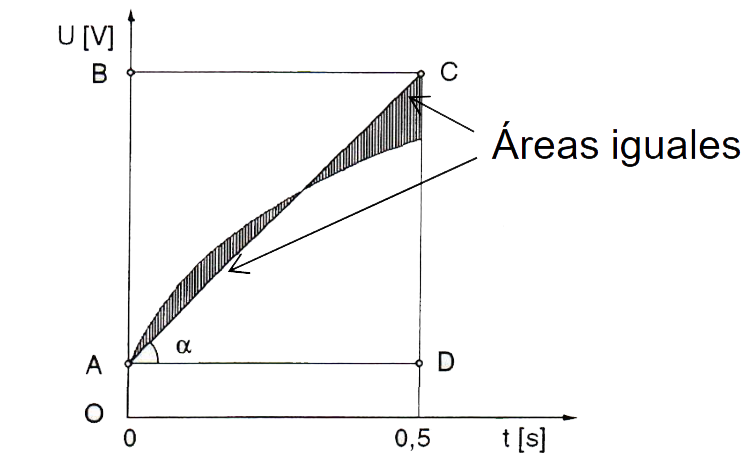
\includegraphics[width=1\linewidth]{res/tema7/tanAlpha}
				\end{minipage}
			\end{figure}
			
			En el caso de un cortocircuito en la red, el inducido provoca un campo opuesto al campo principal, lo que provoca que la excitatriz tiene que suministrar una potencia más alta que en servicio nominal. Este exceso de tensión puede estar entre un 40 y un 80\% de la tensión nominal.
					
		\subsection{Clasificación de los sistemas de excitación.}
			\begin{itemize}
				\item Excitación estática o directa:
					\begin{itemize}
						\item Sistema autoexcitado.
						\item Excitación independiente.
					\end{itemize}
				\item Excitación rotativa o indirecta:
					\begin{itemize}
						\item Excitatriz de c.a. con diodos giratorios.
						\item Excitatriz de c.c.
						\item Excitación independiente o autoexcitada.
						\item Chopper o rectificador de alterna con tiristores.
					\end{itemize}
			\end{itemize}
		
			\newpage
			\subsubsection{Excitación estática o directa, autoexcitada con anillos y escobillas.}

						Es un sistema autoexcitado de excitación independiente. Muy habitual en generadores de pequeña potencia. 
						

						Se alimenta el inductor a través de anillos rozantes y escobillas. Es un sistema de respuesta rápida y es autónomo menos en el arranque. 
						

						Tiene la desventaja de tener una respuesta pobre ante cortocircuitos cercanos.

						\begin{figure}[H]
							\centering
							\begin{circuitikz}
								\tikzstyle{every node}=[font=\normalsize]
								\draw  (13,14.25) circle (0.75cm);
								\draw  (13,13.5) circle (0.75cm);
								\draw  (14.5,11.75) circle (0.5cm);
								\draw  (15,11.75) circle (0.5cm);
								\draw (17.5,10.5) to[D] (16.5,10.5);
								\draw  (16.25,11) rectangle (17.75,10);
								\draw  (13,9.25) circle (1.5cm);
								\draw  (13,9.25) circle (1cm) node {\normalsize Rotor} ;
								\node [font=\normalsize] at (13,7.5) {Estátor};
								\draw [](13,10.75) to[short] (13,12.75);
								\draw[] (14,11.75) to[short] (13,11.75);
								\node at (13,11.75) [circ] {};
								\node [font=\normalsize] at (14.75,12.9) {Transformador};
								\node [font=\normalsize] at (14.75,12.5) {de excitación};
								\node [font=\normalsize, rotate around={90:(0,0)}] at (11.55,14) {Transformador};
								\node [font=\normalsize, rotate around={90:(0,0)}] at (12,14) {de potencia};
								\draw [](13,15) to[short] (13,16);
								\draw [](12.75,15.75) to[short] (13.25,15.75);
								\node [font=\normalsize, rotate around={-360:(0,0)}] at (14.75,15.75) {Red de transporte};
								\node [font=\normalsize, rotate around={-360:(0,0)}] at (15.25,10.6) {Puente de};
								\draw [](15.5,11.75) to[short] (17,11.75);
								\draw [](17,11.75) to[short] (17,11);
								\draw [](17,10) to[short] (17,9.25);
								\draw[] (17,9.25) to[short] (14,9.25);
								\node [font=\normalsize, rotate around={-360:(0,0)}] at (15.25,10.25) {tiristores};
								\node [font=\normalsize, rotate around={-360:(0,0)}] at (16.25,12) {c.a.};
								\node [font=\normalsize, rotate around={-360:(0,0)}] at (15.75,9.5) {c.c.};
								\draw [, rotate around={-360:(19.625, 10.5)}] (19,11) rectangle  node {\normalsize AVR} (20.25,10);
								\draw (19,10.5) to[short] (17.75,10.5);
							\end{circuitikz}
							
							\label{fig:my_label}
						\end{figure}
				
		\subsubsection{Excitación estática o directa, con excitación independiente a través de servicios auxiliares.}

					Se alimenta de la red de servicios auxiliares o similar. 
					

					Muy habitual en generadores de pequeña potencia. Utiliza escobillas y anillos rozantes. Respuesta rápida. 
					

					Tiene la desventaja de tener una respuesta pobre ante cortocircuitos cercanos en la red.

					\begin{figure}[H]
						\centering
							\begin{circuitikz}
								\tikzstyle{every node}=[font=\LARGE]
								\draw  (13,14.25) circle (0.75cm);
								\draw  (13,13.5) circle (0.75cm);
								\draw  (17,13.25) circle (0.5cm);
								\draw  (17,12.75) circle (0.5cm);
								\draw (17.5,10.5) to[D] (16.5,10.5);
								\draw  (16.25,11) rectangle (17.75,10);
								\draw  (13,9.25) circle (1.5cm);
								\draw  (13,9.25) circle (1cm) node {\normalsize Rotor} ;
								\node [font=\normalsize] at (13,7.5) {Estátor};
								\draw [](13,10.75) to[short] (13,12.75);
								\node [font=\normalsize, rotate around={90:(0,0)}] at (15.9,13) {Servicios};
								\node [font=\normalsize, rotate around={90:(0,0)}] at (16.25,13) {auxiliares};
								\node [font=\normalsize, rotate around={90:(0,0)}] at (11.55,14) {Transformador};
								\node [font=\normalsize, rotate around={90:(0,0)}] at (12,14) {de potencia};
								\draw [](13,15) to[short] (13,16);
								\draw [](12.75,15.75) to[short] (13.25,15.75);
								\node [font=\normalsize, rotate around={-360:(0,0)}] at (14.75,15.75) {Red de transporte};
								\node [font=\normalsize, rotate around={-360:(0,0)}] at (15.25,10.6) {Puente de};
								\draw [](17,12.25) to[short] (17,11.75);
								\draw [](17,11.75) to[short] (17,11);
								\draw [](17,10) to[short] (17,9.25);
								\draw[] (17,9.25) to[short] (14,9.25);
								\node [font=\normalsize, rotate around={-360:(0,0)}] at (15.25,10.25) {tiristores};
								\node [font=\normalsize, rotate around={90:(0,0)}] at (16.75,11.75) {c.a.};
								\node [font=\normalsize, rotate around={-360:(0,0)}] at (15.75,9.5) {c.c.};
								\draw [, rotate around={-360:(19.625, 10.5)}] (19,11) rectangle  node {\normalsize AVR} (20.25,10);
								\draw[] (19,10.5) to[short] (17.75,10.5);
								\draw [](17,13.75) to[short] (17,14.5);
							\end{circuitikz}
						
						\label{fig:my_label}
					\end{figure}

		\newpage
			
		\subsubsection{Excitación rotativa o indirecta, con excitatriz de c.c. sin excitatriz piloto.}
					Una máquina de c.c. alimenta el inductor a través de anillos rozantes y escobillas. Unida al eje del generador.
					

					Para generadores hidráulicos de hasta $50\,MV\!A$. 
					

					Alimentación independiente mediante red auxiliar.
					\vspace{0.5cm}
					\begin{figure}[H]
						\centering
							\begin{circuitikz}
								\tikzstyle{every node}=[font=\normalsize]
								\draw  (13,14.25) circle (0.75cm);
								\draw  (13,13.5) circle (0.75cm);
								\draw  (18.5,14) circle (0.5cm);
								\draw  (18.5,13.5) circle (0.5cm);
								\draw (19,11.25) to[D] (18,11.25);
								\draw  (17.75,11.75) rectangle (19.25,10.75);
								\draw  (13,9.25) circle (1.5cm);
								\draw  (13,9.25) circle (1cm) node {\normalsize Generador} ;
								\draw [](13,10.75) to[short] (13,12.75);
								\node [font=\normalsize, rotate around={90:(0,0)}] at (17.4,13.75) {Servicios};
								\node [font=\normalsize, rotate around={90:(0,0)}] at (17.75,13.75) {auxiliares};
								\node [font=\normalsize, rotate around={90:(0,0)}] at (11.55,14) {Transformador};
								\node [font=\normalsize, rotate around={90:(0,0)}] at (12,14) {de potencia};
								\draw [](13,15) to[short] (13,16);
								\draw [](12.75,15.75) to[short] (13.25,15.75);
								\node [font=\normalsize, rotate around={-360:(0,0)}] at (14.75,15.75) {Red de transporte};
								\node [font=\normalsize, rotate around={-360:(0,0)}] at (16.75,11.3) {Puente de};
								\draw [](18.5,13) to[short] (18.5,12.5);
								\draw [](18.5,12.5) to[short] (18.5,11.75);
								\draw [](18.5,10.75) to[short] (18.5,10);
								\node [font=\normalsize, rotate around={-360:(0,0)}] at (16.75,11) {tiristores};
								\node [font=\normalsize, rotate around={90:(0,0)}] at (18.25,12.5) {c.a.};
								\draw [, rotate around={-360:(21.125, 11.25)}] (20.5,11.75) rectangle  node {\normalsize AVR} (21.75,10.75);
								\draw[] (20.5,11.25) to[short] (19.25,11.25);
								\draw [](18.5,14.5) to[short] (18.5,15.25);
								
								\draw  (16.5,9.25) circle (0.5cm);
								\draw  (16.5,9.25) circle (0.75cm) node {\normalsize Exc.} ;
								\draw [dashed] (14,9.25) -- (16,9.25);
								\draw [short] (13.75,9.875) -- (14.5,10.5);
								\draw [short] (13.75,8.625) -- (14.5,8);
								\draw [short] (14.5,10.5) -- (16.5,10.5);
								\draw [short] (16.5,10.5) -- (16.5,10);
								\draw [short] (16.5,8.5) -- (16.5,8);
								\draw [short] (16.5,8) -- (14.5,8);
								\node at (16.5,10) [circ] {};
								\node at (16.5,8.5) [circ] {};
								\draw [ fill={rgb,255:red,0; green,0; blue,0} , rotate around={-360:(17.625, 9.25)}] (17.5,10) rectangle (17.75,8.5);
								\draw [](18.5,10) to[short] (18.5,9.25);
								\draw[] (18.5,9.25) to[short] (17.75,9.25);
								\node [font=\normalsize, rotate around={90:(0,0)}] at (18.25,10) {c.c.};
								\node [font=\normalsize, rotate around={-360:(0,0)}] at (15.25,8.25) {c.c.};
							\end{circuitikz}
						
						\label{fig:my_label}
					\end{figure}
					\vspace{1cm}
		\subsubsection{Excitación rotativa o indirecta, con excitatriz principal y piloto de c.c.}
			Muy habitual en generadores de baja velocidad y media potencia, hasta $50\,MV\!A$.
			
			
			Excitatriz piloto y principal de c.c.
			
			
			Sistema autónomo. No depende de la red, sólo se necesita hacer girar el eje común a las 3 máquinas. Se alimenta a través de anillos y escobillas.
			
			
			Respuesta más lenta y mayor coste de mantenimiento por las escobillas.
			\vspace{0.5cm}
			\begin{figure}[H]
				\centering
				\begin{circuitikz}
					\tikzstyle{every node}=[font=\normalsize]
					\draw  (10,12.75) circle (1.5cm);
					\draw  (10,12.75) circle (1cm);
					\draw (10,13.5) to[L ] (10,12);
					\draw [dashed] (10,12.75) -- (18.5,12.75);
					\draw [ fill={rgb,255:red,0; green,0; blue,0} , rotate around={-360:(12.625, 12.75)}] (12.5,13.25) rectangle (12.75,12.25);
					\draw [ fill={rgb,255:red,0; green,0; blue,0} , rotate around={-360:(13.125, 12.75)}] (13,13.25) rectangle (13.25,12.25);
					\draw  (15,12.75) circle (0.5cm);
					\node at (15,13.25) [circ] {};
					\node at (15,12.25) [circ] {};
					\draw [](10,12) to[short] (11.75,12);
					\draw [](11.75,12) to[short] (11.75,12.25);
					\draw [](11.75,12.25) to[short] (11.75,12.5);
					\draw [](11.75,12.5) to[short] (13,12.5);
					\draw [](10,13.5) to[short] (11.75,13.5);
					\draw [](11.75,13.5) to[short] (11.75,13);
					\draw [](11.75,13) to[short] (12.5,13);
					\draw [](12.625,13.25) to[short] (12.625,13.75);
					\draw [](12.625,13.75) to[short] (15,13.75);
					\draw [](15,13.75) to[short] (15,13.25);
					\draw [](15,12.25) to[short] (15,11.75);
					\draw[] (15,11.75) to[short] (13.125,11.75);
					\draw [](13.125,11.75) to[short] (13.125,12.25);
					\draw (16,13.5) to[L ] (16,12);
					\draw  (18.5,12.75) circle (0.5cm);
					\draw [](18.5,13.25) to[short] (18.5,13.75);
					\draw [](18.5,12.25) to[short] (18.5,11.75);
					\draw (16,13.75) to[R] (17.5,13.75);
					\draw [->, >=Stealth] (16.75,14.5) -- (16.75,14);
					\draw [short] (16.75,14.5) -- (18.5,14.5);
					\draw [short] (18.5,14.5) -- (18.5,13.75);
					\draw [short] (16,13.75) -- (16,13.5);
					\draw [short] (18.5,11.75) -- (16,11.75);
					\draw [short] (16,11.75) -- (16,12);
					\draw (19.5,13.5) to[L ] (19.5,12);
					\draw [](19.5,13.5) to[short] (19.5,14.5);
					\draw[] (19.5,14.5) to[short] (18.5,14.5);
					\draw [](18.5,11.75) to[short] (19.5,11.75);
					\draw [](19.5,11.75) to[short] (19.5,12);
					\node at (18.5,14.5) [circ] {};
					\node at (18.5,11.75) [circ] {};
					\node [font=\normalsize, rotate around={-360:(0,0)}] at (18.25,13.5) {+};
					\node [font=\normalsize, rotate around={-360:(0,0)}] at (14.75,13.5) {+};
					\node [font=\normalsize, rotate around={-360:(0,0)}] at (15.5,11.4) {Excitatriz};
					\node [font=\normalsize, rotate around={-360:(0,0)}] at (15.5,11.1) {principal};
					\node [font=\normalsize, rotate around={-360:(0,0)}] at (19,11.4) {Excitatriz};
					\node [font=\normalsize, rotate around={-360:(0,0)}] at (19,11.1) {piloto};
					\draw (7,12.75) to[tmultiwire= \normalsize Red] (8.5,12.75);
				\end{circuitikz}
				
				\label{fig:my_label}
			\end{figure}
		\newpage
		\subsubsection{Excitación rotativa o indirecta, con excitatriz de c.a. y piloto de imanes permanentes}
			Potencias de hasta $50\,MV\!A$.
			
			
			Se necesitan anillos y escobillas en el alternador principal, pero no en las excitatrices.
			
			
			Sistema autónomo de la red: sólo es necesario girar el eje de la turbina.
			
			
			Tiempo de respuesta lento, coste de mantenimiento alto por las escobillas, y no es aconsejable subir de 1500 $rpm$ por la resistencia mecánica en las escobillas.
			\vspace{0.5cm}
			\begin{figure}[H]
				\centering
				\begin{circuitikz}
					\tikzstyle{every node}=[font=\normalsize]
					\draw  (10,12.75) circle (1.5cm);
					\draw  (10,12.75) circle (1cm);
					\draw (10,13.5) to[L ] (10,12);
					\draw [dashed] (10,12.75) -- (18,12.75);
					\draw [ fill={rgb,255:red,0; green,0; blue,0} , rotate around={-360:(12.625, 12.75)}] (12.5,13.25) rectangle (12.75,12.25);
					\draw [ fill={rgb,255:red,0; green,0; blue,0} , rotate around={-360:(13.125, 12.75)}] (13,13.25) rectangle (13.25,12.25);
					\draw [](10,12) to[short] (11.75,12);
					\draw [](11.75,12) to[short] (11.75,12.25);
					\draw [](11.75,12.25) to[short] (11.75,12.5);
					\draw [](11.75,12.5) to[short] (13,12.5);
					\draw [](10,13.5) to[short] (11.75,13.5);
					\draw [](11.75,13.5) to[short] (11.75,13);
					\draw [](11.75,13) to[short] (12.5,13);
					\draw [](13.125,13.25) to[short] (13.125,14.5);
					\draw [](7,12.75) to[tmultiwire= \normalsize Red] (8.5,12.75);
					\draw (15,14.75) to[D] (14,14.75);
					\draw [, rotate around={-360:(14.5, 14.75)}] (13.75,15.25) rectangle (15.25,14.25);
					\draw [short] (13.125,14.5) -- (13.75,14.5);
					\draw [short] (13.75,15) -- (12.625,15);
					\draw [short] (12.625,15) -- (12.625,13.25);
					\draw [short] (15.25,14.75) -- (16.25,14.75);
					\draw  (16.25,12.75) circle (1cm);
					\draw  (16.25,12.75) circle (1.25cm);
					\draw [](16.25,13.74) to[tmultiwire] (16.25,14.75);
					\draw [](17.25,13.5) to[short] (18,13.5);
					\draw [](17.25,12) to[short] (18,12);
					\draw (18.5,12.25) to[D] (18.5,13.25);
					\draw [, rotate around={-360:(18.5, 12.75)}] (18,13.75) rectangle (19,11.75);
					\draw [dashed] (19,12.75) -- (20.5,12.75);
					\draw  (21,12.75) circle (0.75cm) node {\normalsize G} ;
					\draw  (21,12.75) circle (0.5cm);
					\draw[] (21,14.25) to[tmultiwire] (18.5,14.25);
					\draw [](21,14.25) to[short] (21,13.5);
					\draw [](18.5,14.25) to[short] (18.5,13.75);
					\node [font=\normalsize, rotate around={-360:(0,0)}] at (16.75,11.25) {Excitatriz principal};
					\node [font=\normalsize, rotate around={-360:(0,0)}] at (16.75,10.85) {de corriente alterna};
					\node [font=\normalsize, rotate around={-360:(0,0)}] at (21,11.25) {Excitatriz piloto};
					\node [font=\normalsize, rotate around={-360:(0,0)}] at (21,10.8) {de imanes permanentes};
					\node [font=\normalsize, rotate around={-360:(0,0)}] at (10,11) {Alternador};
				\end{circuitikz}
				
				\label{fig:my_label}
			\end{figure}
		
		
		\subsubsection{Excitación rotativa o indirecta, con generador auxiliar de c.a. de imanes permanentes.}

					Potencias de hasta $50\,MV\!A$.
					

					Se alimenta el inductor con una excitatriz de imanes permanentes de c.a acoplada en el mismo eje. Al ser de imanes permanentes el flujo en la excitatriz es constante. El inductor del generador síncrono se alimenta a través de escobillas y anillos rozantes.
					

					Sistema más rápido de actuación. Autónomo, pues sólo se necesita mover el eje con la turbina.
					\vspace{0.5cm}
					\begin{figure}[H]
						\centering
						\begin{circuitikz}
							\tikzstyle{every node}=[font=\normalsize]
							\draw  (13,14.25) circle (0.75cm);
							\draw  (13,13.5) circle (0.75cm);
							\draw (16.75,11.25) to[D] (15.75,11.25);
							\draw  (15.5,11.75) rectangle (17,10.75);
							\draw  (13,9.25) circle (1.5cm);
							\draw  (13,9.25) circle (1cm) node {\normalsize Generador} ;
							\draw [](13,10.75) to[short] (13,12.75);
							\node [font=\normalsize, rotate around={90:(0,0)}] at (11.55,14) {Transformador};
							\node [font=\normalsize, rotate around={90:(0,0)}] at (12,14) {de potencia};
							\draw [](13,15) to[short] (13,16);
							\draw [](12.75,15.75) to[short] (13.25,15.75);
							\node [font=\normalsize, rotate around={-360:(0,0)}] at (14.75,15.75) {Red de transporte};
							\node [font=\normalsize, rotate around={-360:(0,0)}] at (16.25,10.5) {Puente de};
							\node [font=\normalsize, rotate around={-360:(0,0)}] at (16.25,10.175) {tiristores};
							
							\draw  (19.5,9.25) circle (0.5cm);
							\draw  (19.5,9.25) circle (0.75cm) node {\normalsize G} ;
							\draw [dashed] (14,9.25) -- (19,9.25);
							\draw [short] (13.75,9.875) -- (15,11.25);
							\draw [short] (15,11.25) -- (15.5,11.25);
							\draw [short] (17,11.25) -- (17.5,11.25);
							\draw [short] (17.5,11.25) -- (18.95,9.75);
							\draw [, rotate around={-360:(16.25, 12.75)}] (15.5,13.25) rectangle  node {\normalsize AVR} (17,12.25);
							\draw [](16.25,12.25) to[short] (16.25,11.75);
							\node [font=\normalsize, rotate around={-360:(0,0)}] at (19.5,10.75) {Imanes};
							\node [font=\normalsize, rotate around={-360:(0,0)}] at (19.5,10.5) {Permanentes};
						\end{circuitikz}
						
						\label{fig:my_label}
					\end{figure}

		\newpage
		\subsubsection{Excitación rotativa o indirecta, sin escobillas con diodos giratorios y excitatriz de c.a.}
			Para generadores de alta potencia y respuesta rápida.
			
			
			El inductor del generador, la caja de diodos y el inductor de c.a. de la excitatriz están en el mismo eje. El devanado de excitación de la excitatriz de corriente alterna se alimenta mediante una red independiente o auxiliar.
			
			
			Tiene el inconveniente de dar una respuesta pobre ante cortocircuitos en la red auxiliar.
			
			\vspace{0.25cm}
			\textbf{\textit{Diodos giratorios:}}
			\begin{itemize}
				\item Giran solidarios al eje.
				\item El eje del generado es hueco para poder pasar los cables que vienen del puente rectificador.
				\item La excitatriz principal genera una tensión trifásica con una frecuencia del orden de los $350\,Hz$, para disminuir el rizado. La excitatriz piloto de c.a. genera una tensión trifásica con una frecuencia del orden de los $250\,Hz$.
				\item El puente rectificador de diodos giratorios puede contener cerca de 60 diodos rectificadores, montados en serie y paralelo. Cada diodo lleva asociado un fusible de protección contra cortocircuitos, y puede haber 30 grupos R-C de protección contra sobretensiones.
			\end{itemize}
			
			\begin{figure}[H]
				\centering
					\begin{circuitikz}
						\tikzstyle{every node}=[font=\normalsize]
						\draw  (13,14.25) circle (0.75cm);
						\draw  (13,13.5) circle (0.75cm);
						\draw  (19.75,14) circle (0.5cm);
						\draw  (19.75,13.5) circle (0.5cm);
						\draw (20.25,11.25) to[D] (19.25,11.25);
						\draw  (19,11.75) rectangle (20.5,10.75);
						\draw  (13,9.25) circle (1.5cm);
						\draw  (13,9.25) circle (1cm) node {\normalsize Generador} ;
						\draw [](13,10.75) to[short] (13,12.75);
						\node [font=\normalsize, rotate around={90:(0,0)}] at (18.7,13.75) {Servicios};
						\node [font=\normalsize, rotate around={90:(0,0)}] at (19,13.75) {auxiliares};
						\node [font=\normalsize, rotate around={90:(0,0)}] at (11.65,14) {Transformador};
						\node [font=\normalsize, rotate around={90:(0,0)}] at (12,14) {de potencia};
						\draw [](13,15) to[short] (13,16);
						\draw [](12.75,15.75) to[short] (13.25,15.75);
						\node [font=\normalsize, rotate around={-360:(0,0)}] at (14.75,15.75) {Red de transporte};
						\node [font=\normalsize, rotate around={-360:(0,0)}] at (18,11.3) {Puente de};
						\draw [](19.75,13) to[short] (19.75,12.5);
						\draw [](19.75,12.5) to[short] (19.75,11.75);
						\draw [](19.75,10.75) to[short] (19.75,10);
						\node [font=\normalsize, rotate around={-360:(0,0)}] at (18,11) {tiristores};
						\node [font=\normalsize, rotate around={90:(0,0)}] at (19.5,12.5) {c.a.};
						\draw [, rotate around={-360:(22.375, 11.25)}] (21.75,11.75) rectangle  node {\normalsize AVR} (23,10.75);
						\draw[] (21.75,11.25) to[short] (20.5,11.25);
						\draw [](19.75,14.5) to[short] (19.75,15.25);
						
						\draw  (18.25,9.25) circle (0.5cm);
						\draw  (18.25,9.25) circle (0.75cm) node {\normalsize Exc.} ;
						\draw [short] (14,9.25) -- (15.25,9.25);
						\draw [](19.75,10) to[short] (19.75,9.25);
						\draw[] (19.75,9.25) to[short] (19,9.25);
						\node [font=\normalsize, rotate around={90:(0,0)}] at (19.5,10) {c.c.};
						\draw  (15.25,9.75) rectangle (16.75,8.75);
						\draw (16.5,9.25) to[D] (15.5,9.25);
						\draw [](16.75,9.25) to[short] (17.75,9.25);
						\node [font=\normalsize, rotate around={-360:(0,0)}] at (16,10.5) {Caja de};
						\node [font=\normalsize, rotate around={-360:(0,0)}] at (16,10.15) {diodos giratorios};
						\node [font=\normalsize, rotate around={-360:(0,0)}] at (17.2,9.5) {c.a.};
						\node [font=\normalsize, rotate around={-360:(0,0)}] at (14.85,9.5) {c.c.};
					\end{circuitikz}
				
				\label{fig:my_label}
			\end{figure}
		
		\subsubsection{Excitación rotativa o indirecta, con diodos giratorios, excitatriz de c.a. y excitatriz piloto de imanes permanentes.}
			Sistema de excitación para generadores de alta potencia de respuesta un poco más lenta. 
			
			
			El inductor del generador síncrono, la caja de diodos giratorios y el inductor de c.a de la excitatriz principal están en el mismo eje. El devanado de excitación de la excitatriz de corriente alterna se alimenta mediante un generador de imanes permanentes (flujo constante). El inductor del generador no tiene escobillas ni anillos rozantes. Se alimenta mediante los diodos rectificadores giratorios, a través del eje del generador que está hueco.
			
			
			Sistema autónomo de la red. No le influyen los cortocircuitos en la red.
			
			\begin{figure}[H]
				\centering
				\begin{circuitikz}
					\tikzstyle{every node}=[font=\normalsize]
					\draw (22.75,10.5) to[D] (21.75,10.5);
					\draw  (21.5,11) rectangle (23,10);
					\draw  (13,9.75) circle (1.5cm);
					\draw  (13,9.75) circle (1cm) node {\normalsize Generador} ;
					\node [font=\normalsize, rotate around={-360:(0,0)}] at (24,11.25) {Puente de tiristores};
					
					\draw  (18.25,9.75) circle (0.5cm);
					\draw  (18.25,9.75) circle (0.75cm) node {\normalsize Exc.} ;
					\draw [short] (14,9.75) -- (15.25,9.75);
					\draw[] (21.5,10.5) to[short] (21,10.5);
					\node [font=\normalsize, rotate around={-360:(0,0)}] at (20.75,10.75) {c.c.};
					\draw  (15.25,10.25) rectangle (16.75,9.25);
					\draw (16.5,9.75) to[D] (15.5,9.75);
					\draw [](16.75,9.75) to[short] (17.75,9.75);
					\node [font=\normalsize, rotate around={-360:(0,0)}] at (16,8.75) {Caja de};
					\node [font=\normalsize, rotate around={-360:(0,0)}] at (16,8.375) {diodos giratorios};
					\node [font=\normalsize, rotate around={-360:(0,0)}] at (17.2,9.5) {c.a.};
					\node [font=\normalsize, rotate around={-360:(0,0)}] at (14.85,9.5) {c.c.};
					\draw  (10.25,9.75) circle (0.5cm) node {\normalsize M} ;
					\draw [dashed] (10.75,9.75) -- (12,9.75);
					\draw  (21.5,12.25) rectangle  node {\normalsize AVR} (23,11.5);
					\draw [short] (22.25,11.5) -- (22.25,11);
					\draw (19,9.75) to[R] (21,9.75);
					\draw [->, >=Stealth] (20,10.5) -- (20,10);
					\draw [short] (20,10.5) -- (21,10.5);
					\draw [](13,11.25) to[tmultiwire= \normalsize Red] (13,12.25);
					\draw  (24.5,9.75) circle (0.5cm) node {\normalsize G} ;
					\draw [dashed] (24,9.75) -- (21.25,9.75);
					\draw [](23,10.5) to[tmultiwire] (24.5,10.5);
					\draw [](24.5,10.5) to[short] (24.5,10.25);
					\node [font=\normalsize] at (10.25,11) {Motor};
					\node [font=\normalsize] at (10.25,10.625) {primario};
					\node [font=\normalsize] at (24.5,9) {Excitatriz piloto};
					\node [font=\normalsize] at (24.5,8.625) {de imanes permanentes};
					\node [font=\normalsize] at (18.25,11.5) {Excitatriz principal};
					\node [font=\normalsize] at (18.25,11.125) {de corriente};
					\node [font=\normalsize] at (18.25,10.75) {alterna};
				\end{circuitikz}
				
				\label{fig:my_label}
			\end{figure}
		
		\subsubsection{Sistema de autoexcitación con excitatriz de c.a. y diodos giratorios.}
			Muy habitual en generadores de gran potencia.
		
		
			El sistema de excitación se alimenta de la tensión en bornes del generador a través del transformador trifásico de excitación, que alimenta el puente controlado de tiristores o IGBTs.
		
			
			Sistema autónomo, salvo en los arranques. Respuesta rápida.
			
			
			Respuesta pobre cuando hay cortocircuitos cercanos en la red.
			
			
			\vspace{0.25cm}
			\textbf{\textit{Proceso de arranque:}}
			
			
			Dado que el regulador de tensión (AVR) no puede funcionar con la pequeña tensión generada por el magnetismo remanente del generador síncrono, es necesario disponer de una fuente de alimentación independiente que alimente el inductor del generador solamente durante el proceso de arranque.
			
			
			Puede hacerse mediante baterías o una red auxiliar independiente, con un transformador de arranque.
					
			\begin{figure}[H]
				\centering
				\begin{circuitikz}
					\tikzstyle{every node}=[font=\normalsize]
					\draw  (13,14.25) circle (0.75cm);
					\draw  (13,13.5) circle (0.75cm);
					\draw  (15.75,12) circle (0.5cm);
					\draw  (16.25,12) circle (0.5cm);
					\draw (20.25,10.75) to[D] (19.25,10.75);
					\draw  (19,11.25) rectangle (20.5,10.25);
					\draw  (13,9.25) circle (1.5cm);
					\draw  (13,9.25) circle (1cm) node {\normalsize Generador} ;
					\draw [](13,10.75) to[short] (13,12.75);
					\node [font=\normalsize, rotate around={-360:(0,0)}] at (16,13.1) {Transformador};
					\node [font=\normalsize, rotate around={-360:(0,0)}] at (16,12.75) {de excitación};
					\node [font=\normalsize, rotate around={90:(0,0)}] at (11.65,14) {Transformador};
					\node [font=\normalsize, rotate around={90:(0,0)}] at (12,14) {de potencia};
					\draw [](13,15) to[short] (13,16);
					\draw [](12.75,15.75) to[short] (13.25,15.75);
					\node [font=\normalsize, rotate around={-360:(0,0)}] at (14.75,15.75) {Red de transporte};
					\node [font=\normalsize, rotate around={-360:(0,0)}] at (18,11) {Puente de};
					\draw [](19.75,12) to[short] (19.75,11.25);
					\draw [](19.75,10.25) to[short] (19.75,10);
					\node [font=\normalsize, rotate around={-360:(0,0)}] at (18,10.6) {tiristores};
					\node [font=\normalsize, rotate around={-360:(0,0)}] at (18.25,12.25) {c.a.};
					\draw [, rotate around={-360:(22.375, 10.75)}] (21.75,11.25) rectangle  node {\normalsize AVR} (23,10.25);
					\draw[] (21.75,10.75) to[short] (20.5,10.75);
					
					\draw  (18.25,9.25) circle (0.5cm);
					\draw  (18.25,9.25) circle (0.75cm) node {\normalsize Exc.} ;
					\draw [short] (14,9.25) -- (15.25,9.25);
					\draw [](19.75,10) to[short] (19.75,9.25);
					\draw[] (19.75,9.25) to[short] (19,9.25);
					\node [font=\normalsize, rotate around={90:(0,0)}] at (19.5,9.75) {c.c.};
					\draw  (15.25,9.75) rectangle (16.75,8.75);
					\draw (16.5,9.25) to[D] (15.5,9.25);
					\draw [](16.75,9.25) to[short] (17.75,9.25);
					\node [font=\normalsize, rotate around={-360:(0,0)}] at (16,10.5) {Caja de};
					\node [font=\normalsize, rotate around={-360:(0,0)}] at (16,10.15) {diodos giratorios};
					\node [font=\normalsize, rotate around={-360:(0,0)}] at (17.2,9.5) {c.a.};
					\node [font=\normalsize, rotate around={-360:(0,0)}] at (14.85,9.5) {c.c.};
					\draw [](16.75,12) to[short] (19.75,12);
					\draw[] (15.25,12) to[short] (13,12);
					\node at (13,12) [circ] {};
				\end{circuitikz}
				
				\label{fig:my_label}
			\end{figure}
		
	\subsection{Cortocircuitos en la red.}	
		Constituye un problema importante, pues en este caso la tensión de alimentación de la excitación desaparece total o parcialmente, en función de la impedancia que pueda haber entre el generador y el punto de defecto.
		
		
		Si el alternador está conectado directamente a un juego de barras, del que se alimentan una serie de cargas y se produce un cortocircuito en una de las líneas, ésta debe ser automáticamente desconectada de forma selectiva y en un tiempo muy breve a fin de no dejar sin suministro el resto de las cargas. En el caso de un alternador autoexcitado, la $I_{cc}$ decrece rápidamente debido a la reducción de la $I_{ex}$ provocada por la reducción de la tensión.
		
	\section{Regulador de tensión (AVR).}
		Tiene como misión:
		\begin{itemize}
			\item Mantener la tensión en bornes del generador dentro de los márgenes permitidos, independientemente del nivel de carga. Normalmente $\pm5\%$ de la tensión nominal.
			\item Regular la potencia reactiva, subexcitando y sobreexcitando al alternador. El generador debe ser capaz de dar un $\pm15\%$ de la potencia activa neta en reactiva.
			\item Mantener el sincronismo del alternador con la red en el caso de un cortocircuito.
			\item Funciones de protección para no sobrepasar los límites de funcionamiento de la máquina.
		\end{itemize}
		
		\subsection{Funciones de regulación y protección del AVR.}
			\begin{itemize}
				\item \textbf{Limitación por excitación máxima.} Evita el sobrecalientamiento del devanado de campo debido a una sobrecorriente.
				\item \textbf{Limitación por excitación mínima.} Evita que la excitación descienda por debajo de un nivel que desestabilice el generador.
				\item \textbf{Limitación y protección V/Hz.} Protege a la instalación contra un flujo magnético elevado que pueda provocar el sobrecalentamiento del circuito magnético. $\dfrac{V}{Hz} \propto \Phi_m$
				\item \textbf{Protección contra cortocircuitos del devanado de campo.} Evita una corriente negativa en el devanado de campo o bien una tensión excesiva en el mismo debida a un cortocircuito en la red. Esta protección proporciona un paso alternativo para la corriente, actuando como un cortocircuito del devanado de campo. Este camino puede abrirse a través de un tiristor que permita el paso de corriente a través de una resistencia de descarga, o también a través de una resistencia no lineal o varistor.
				\item \textbf{Sensado de tensión y compensación de carga.} Mide la tensión en los terminales del generador, la rectifica, la filtra, y una vez convertida en una señal de corriente continua la compara con una referencia que representa la tensión deseada. Además, puede compensar la caída de tensión en el circuito de salida, con el fin de controlar la tensión en un punto distinto de las bornes del generador.
				\item \textbf{Limitación del ángulo de par.} Se fija un máximo entre $80$ y $85^\circ$. El valor del ángulo del par $\delta$ se haya comparando la tensión en b.g. y en b.c.
			\end{itemize}
			
	\section{Esquema de control. Modelado del grupo de generación.}
		Función de transferencia en lazo abierto ($a$ = amplificador, $e$ = excitatriz, $g$ = generador):
		\begin{figure}[H]
			\centering
				\begin{circuitikz}
					\tikzstyle{every node}=[font=\normalsize]
					\draw [->, >=Stealth] (6,13) -- (7.25,13)node[pos=0.4,above]{$\Delta e$};
					\draw  (7.25,13.5) rectangle  node {\normalsize $G_a(s)$} (8.5,12.5);
					\draw  (9.75,13.5) rectangle  node {\normalsize $G_e(s)$} (11,12.5);
					\draw  (12.25,13.5) rectangle  node {\normalsize $G_g(s)$} (13.5,12.5);
					\draw [->, >=Stealth] (8.5,13) -- (9.75,13)node[pos=0.5,above]{$\Delta V_R$};
					\draw [->, >=Stealth] (11,13) -- (12.25,13)node[pos=0.5,above]{$\Delta V_f$};
					\draw [->, >=Stealth] (13.5,13) -- (14.75,13)node[pos=0.5,above]{$\Delta |V|$};
					\draw [->, >=Stealth] (6,11.5) -- (7.25,11.5)node[pos=0.4,above]{$\Delta e$};
					\draw  (7.25,12) rectangle  node {\normalsize $\dfrac{K_a}{1+sT_a}$} (8.75,11);
					\draw  (10,12) rectangle  node {\normalsize $\dfrac{K_e}{1+sT_e}$} (11.5,11);
					\draw  (12.75,12) rectangle  node {\normalsize $\dfrac{K_g}{1+sT_g}$} (14.25,11);
					\draw [->, >=Stealth] (8.75,11.5) -- (10,11.5)node[pos=0.5,above]{$\Delta V_R$};
					\draw [->, >=Stealth] (11.5,11.5) -- (12.75,11.5)node[pos=0.5,above]{$\Delta V_f$};
					\draw [->, >=Stealth] (14.25,11.5) -- (15.5,11.5)node[pos=0.5,above]{$\Delta |V|$};
				\end{circuitikz}
			
			\label{fig:my_label}
		\end{figure}
		
		Se modelan todos los componentes como sistemas de primer orden, por lo tanto la función de transferencia en lazo abierto final tendrá 3 polos:
		\begin{figure}[H]
			\centering
				\begin{circuitikz}
					\tikzstyle{every node}=[font=\normalsize]
					\draw [->, >=Stealth] (8,8.25) -- (9.25,8.25)node[pos=0.4,above]{$\Delta e$};
					\draw [->, >=Stealth] (14,8.25) -- (15.25,8.25)node[pos=0.5,above]{$\Delta |V|$};
					\draw  (9.25,8.75) rectangle  node {\normalsize $\dfrac{K_a K_e K_g}{(1+sT_a)(1+sT_e)(1+sT_g)}$} (14,7.75);
				\end{circuitikz}
			
			\label{fig:my_label}
		\end{figure}
		
		
		Cerrando el lazo resulta:
		
		\begin{figure}[H]
			\centering
				\begin{circuitikz}
					\tikzstyle{every node}=[font=\normalsize]
					\draw [->, >=Stealth] (8,8.25) -- (9.25,8.25)node[pos=0.4,above]{$\Delta e$};
					\draw [->, >=Stealth] (14,8.25) -- (15.5,8.25)node[pos=0.5,above]{$\Delta |V|$};
					\draw  (9.25,8.75) rectangle  node {\normalsize $\dfrac{K_aK_eK_g}{(1+sT_a)(1+sT_e)(1+sT_g)}$} (14,7.75);
					\draw  (7.75,8.25) circle (0.25cm);
					\draw [->, >=Stealth] (7.75,7.25) -- (7.75,8);
					\draw [short] (7.75,7.25) -- (14.75,7.25);
					\draw [short] (14.75,7.25) -- (14.75,8.25);
					\node at (14.75,8.25) [circ] {};
					\draw [->, >=Stealth] (6.5,8.25) -- (7.5,8.25)node[pos=0,above]{$\Delta |V_{ref}|$};
					\node [font=\normalsize] at (7.25,8.5) {+};
					\node [font=\normalsize] at (8,7.75) {-};
				\end{circuitikz}
			
			\label{fig:my_label}
		\end{figure}
		
		Donde $T_a < T_e < T_g$, luego el polo del amplificador será el más lento y el del generador el más rápido.
		
		\newpage
		\begin{figure}[H]
			\begin{minipage}{0.29\textwidth}
				Es necesario cuidar el valor de la ganancia total. Visualizándolos en el lugar de las raíces de la figura adjunta. Se observa que para un valor de $K$ muy alto el sistema puede volverse inestable. El AVR tiene en cuenta esto con los parámetros que se describieron en el apartado de "funciones de regulación".				
			\end{minipage}
			\begin{minipage}{0.7\textwidth}
				\begin{figure}[H]
					\centering
					\begin{circuitikz}
						\tikzstyle{every node}=[font=\normalsize]
						\draw [->, >=Stealth] (12.75,4.75) -- (12.75,10.25)node[pos=1,right]{$j\omega$};
						\draw [->, >=Stealth] (9,7.5) -- (14.5,7.5)node[pos=1,right]{$\sigma$};
						\node at (12.25,7.5) [] {$\times$};
						\node at (10.75,7.5) [] {$\times$};
						\node at (9,7.5) [] {$\times$};
						\node [font=\footnotesize] at (9,7) {$s=-\dfrac{1}{T_a}$};
						\node [font=\footnotesize] at (10.5,7) {$s=-\dfrac{1}{T_e}$};
						\node [font=\footnotesize] at (12,7) {$s=-\dfrac{1}{T_g}$};
						\draw [ color={rgb,255:red,0; green,128; blue,255}, short] (9,7.5) -- (7.75,7.5);
						\draw [ color={rgb,255:red,0; green,128; blue,255}, short] (13.5,10.25) .. controls (11.25,8) and (11.25,6.75) .. (13.5,4.75);
						\node at (13,5.25) [, color={rgb,255:red,0; green,128; blue,255}] {\scriptsize$\bigtriangleup$};
						\node at (13,9.75) [, color={rgb,255:red,0; green,128; blue,255}] {\scriptsize$\bigtriangleup$};
						\node at (8.25,7.5) [, color={rgb,255:red,0; green,128; blue,255}] {\scriptsize$\bigtriangleup$};
						\draw [ color={rgb,255:red,0; green,128; blue,255}, dashed] (13,9.75) -- (13,5.25);
						\node [font=\normalsize, color={rgb,255:red,0; green,128; blue,255}] at (8.25,7.75) {$s_1$};
						\node [font=\normalsize, color={rgb,255:red,0; green,128; blue,255}] at (13.35,9.75) {$s_2$};
						\node [font=\normalsize, color={rgb,255:red,0; green,128; blue,255}] at (13.35,5.25) {$s_3$};
						\normalsize
						\draw [ color={rgb,255:red,255; green,0; blue,0}, ->, >=Stealth, dashed] (12.75,10.5) -- (14.25,10.5)node[pos=0.5,above]{Inestable};
						\draw [ color={rgb,255:red,0; green,128; blue,0}, ->, >=Stealth, dashed] (12.75,10.5) -- (11.25,10.5)node[pos=0.5,above]{Estable};
						\draw [ color={rgb,255:red,255; green,0; blue,0}, ->, >=Stealth, dashed] (14.25,8) -- (13.25,9.5)node[pos=0,right]{Polos inestables};
						\draw [ color={rgb,255:red,255; green,0; blue,0}, ->, >=Stealth, dashed] (14.25,8) -- (13.25,5.5);
						\draw [ color={rgb,255:red,0; green,128; blue,255}, short] (10.75,7.5) -- (12.25,7.5);
					\end{circuitikz}
					
					\label{fig:my_label}
				\end{figure}
			\end{minipage}
		\end{figure}	
	
		\subsection{Estructura del control V-Q del sistema eléctrico de potencia.}
			\begin{itemize}
				\item \textbf{Control primario a nivel de central:}
					\begin{itemize}
						\item Sistema de excitación del generador. Regulación de tensión.
						\item Compensación síncrona.
						\item Tomas de regulación en el transformador de potencia.
					\end{itemize}
				\item \textbf{Control secundario en subestaciones:}
					\begin{itemize}
						\item Baterías de condensadores y reactancias conectadas en paralelo.
						\item Compensadores estáticos.
						\item Transformadores reguladores.
						\item Compensadores síncronos permanentemente conectados (líneas largas).
					\end{itemize}
				\item \textbf{Control terciario o nacional:}
					\begin{itemize}
						\item Servicios complementarios.
						\item Control de tensión en la red.
						\item Participación selectiva.
						\item Retribuido.
					\end{itemize}
			\end{itemize}
		
		\subsection{Control primario a nivel de central.}
			Comprende el nivel de control de la tensión en bornes de los generadores constituidos por los reguladores (AVRs) y el control de la tensión en barras de la central o regulador de planta (PQRs).
			
			
			El margen de variación de tensión que típicamente admite un generador en bornes es de $\pm5\%$ con respecto a su tensión nominal.
			
			
			El tiempo de respuesta está fijado alrededor de un minuto el tiempo de variación de la tensión de generador desde el valor mínimo ($-5\%$, valor máximo de absorción de reactiva [\textit{lagging}]) al valor máximo ($+5\%$, valor máximo de generación de reactiva [\textit{leading}]).
			
			
			\subsubsection{Regulador de central: PQR.}
				El objetivo de los PQRs es repartir equilibradamente la generación de reactiva entre los diferentes grupos de la central y alcanzar la consigna de tensión y/o de potencia reactiva que reciba del nivel de control jerárquicamente superior. Los AVRs se pueden controlar mediante señal local o remota de los PQRs.
				
				
				La ley de control del PQR está basada en la resolución de un problema de optimización, y minimiza el error en régimen permanente de la tensión de alta o en barras de la central y de la generación de reactiva total.
				
				
				Los PQRs mantienen en barras de la central las consignas de tensión y/o la generación o absorción de reactiva, modificando la consigna de tensión a la salida de los grupos bajo control. Están coordinados con los RVRs.
				
				
				Disponen de dos canales de control: manual y automático (recibe consignas del control secundario).
				
				\vspace{0.25cm}
				\textit{\textbf{Funciones:}}
				\begin{itemize}
					\item Reparte equitativamente la generación de potencia reactiva entre los grupos de la central según sus límites.
					\item Se asegura el mantenimiento de las tensiones y reactiva de los grupos y servicios auxiliares dentro de los
					límites operativos.
					\item Se adapta a procedimientos de operación de REE.
					\item Incentiva la preferencia por la central, situándola en una situación óptima para que sus recursos sean
					asignados y se obtenga una mayor retribución.
				\end{itemize}
				
				
				\textbf{\textit{Optimización:}}
				
				
					El proceso de optimización está sujeto a los límites de los grupos y de control del PQR:
					\begin{itemize}
						\item Límite máximo y mínimo de tensión de grupo.
						\item Límite máximo y mínimo de tensión de los servicios auxiliares.
						\item Límite máximo y mínimo de absorción de reactiva.
						\item Límite máximo de incremento de consigna en un paso de control.
						\item Máximo desequilibrio de reactiva entre los grupos. Normalmente nulo.
					\end{itemize}
					Si se requiere una variación mayor se utiliza el transformador principal de potencia con regulador de tomas en alta tensión y en carga.
					
			\subsubsection{Control mediante tomas de regulación del transformador.}
				Los transformadores con cambio de tomas contienen un devanado en el que la conexión puede realizarse a lo largo de distintos puntos, permitiendo una regulación directa de la relación de transformación dentro de un margen relativamente estrecho. El margen de regulación típico es $\pm10\%$ respecto a la relación de transformación nominal o la tensión nominal. Este margen suele estar dividido en escalones de aproximadamente $\pm2\%$. Por ejemplo, un transformador de $400/21\,kV$ $\pm 16 \pm 0.8\%$, es decir, 32 tomas de $0.8\,kV$.
				
				\vspace{0.25cm}
				\textbf{\textit{Casuísticas según las tensiones del transformador:}}
				\begin{itemize}
					\item Al aumentar la relación de transformación aumenta la potencia reactiva que pasa por el transformador:
					\[\uparrow U_2 \Rightarrow \downarrow U_1' \Rightarrow U_1 > U_1' \Rightarrow \text{Fluye Q hacia la red.}\]
					\item $U_1' > U_2$: la potencia reactiva fluye desde el generador hacia la red $\Rightarrow$ Red inductiva, generador sobreexcitado.
					\item $U_1' < U_2$: la potencia reactiva fluye desde la red hacia el generador $\Rightarrow$ Red capacitiva, generador subexcitado.
				\end{itemize}
				
			\subsubsection{Compensadores síncronos.}
				Pueden estar instalados en la central o en subestaciones primarias. Son máquinas síncronas funcionando como motor $(\delta < 0)$. Consumen potencia activa y pueden generar o absorber reactiva. Hay que utilizar otra máquina para sincronizarlos a la red.
				
				
				A diferencia de los compensadores estáticos (SVCs):
				\begin{itemize}
					\item Puede regular la tensión de forma continua, sin transitorios.
					\item No introduce ni se ve afectado por armónicos en la red.
					\item No causa problemas de resonancia.
					\item En casos de caída de tensión son capaces de proporcionar corriente de cortocircuito durante un tiempo limitado, facilitando el ajuste de las protecciones de sobreintensidad.
				\end{itemize}
				
		\subsection{Control secundario.}
		\subsubsection{Control zonal (RVR).}
			Se sitúa entre el nivel de control de minimización de pérdidas y el nivel de control de central. Actúa en un tiempo entre 20 segundos a 2 minutos.
			
			
			Para cada zona de control, se definen unos nudos pilotos en los cuales se desea mantener un perfil de tensiones. El RVR mantiene las tensiones de dichos nudos en sus valores de consigna y dentro de la tolerancia permitida $\pm7\%$ (redes de transporte de 400 y 220 kV). El RVR dispone de todos los datos de tensiones y potencias reactivas del sistema eléctrico de potencia de cada zona. Está diseñado para seguir las variaciones de demanda y los cambios diarios en el sistema.
			
			
			Intercambia información con los PQRs y entre los RVRs de otras zonas. Envían información cada diez minutos a los RVRs de tal forma que los RVRs conocen las capacidades reales de cada central.
			
			\vspace{0.25cm}
			\textit{\textbf{Nudo piloto típico:}}
			\begin{figure}[H]
				\begin{minipage}{0.35\textwidth}
					\begin{figure}[H]
						\centering
						\begin{circuitikz}
							\tikzstyle{every node}=[font=\normalsize]
							\draw  (11.5,15.25) circle (0.5cm) node {\normalsize G} ;
							\draw [short] (11.5,14.75) -- (11.5,14.25);
							\draw [short] (10.75,14.25) -- (12.25,14.25);
							\draw [->, >=Stealth] (11,14.25) -- (11,13.25)node[pos=1,left]{$P_{dk}+jQ_{dk}$};
							\draw [->, >=Stealth] (12,14.25) -- (12,13.25)node[pos=1,right]{$U_k$};
							\node [font=\normalsize] at (12.75,14.5) {$P_{gk}+jQ_{gk}$};
							\node [font=\normalsize] at (10,14.25) {Nudo $k$};
						\end{circuitikz}
						
					\end{figure}
				\end{minipage}
				\hspace{0.25cm}
				\begin{minipage}{0.6\textwidth}
					\textbf{\textit{Datos:}}
					
					$Q_{max}$ y $Q_{min}$ que se puede inyectar o absorber en el nudo.
					
					$P_{gk} - P_{dk} = P_k$ (pérdidas).
					
					$U_k$ dentro de unos límites.
				\end{minipage}
			\end{figure}
			
			\subsubsection{Estabilidad de tensión en los nudos.}
			\vspace{-0.6cm}
				\begin{figure}[H]
					\begin{minipage}{0.35\textwidth}
						Las tensiones en los nudos deben mantenerse estables y dentro de sus límites aceptables. Con cargas pequeñas (menor consumo de reactiva), la tendencia de la tensión es a subir cuando la carga es capacitiva y a bajar cuando la carga es inductiva. Sin embargo, con cargas grandes (mayor consumo de reactiva) la tensión siempre decrece.
						
						\vspace{0.25cm}
						Las curvas P-V, o curvas nariz, se pueden obtener para los diferentes nudos de control. Los puntos situados por debajo de la línea discontinua son inestables y el sistema eléctrico nunca opera en ellos.
					\end{minipage}
					\hspace{0.15cm}
					\begin{minipage}{0.6\textwidth}
						\begin{figure}[H]
							\centering
							\begin{circuitikz}[scale = 0.7]
								\tikzstyle{every node}=[font=\normalsize]
								\draw [->, >=Stealth] (9.5,9) -- (9.5,19);
								\draw [->, >=Stealth] (9,9.5) -- (21.5,9.5);
								\draw [ color={rgb,255:red,0; green,128; blue,255}, short] (9.5,18.5) .. controls (26,19.25) and (24.25,13) .. (9.75,9.75);
								\draw [ color={rgb,255:red,0; green,128; blue,255}, short] (9.5,18.5) .. controls (21,18.25) and (24.75,14.75) .. (9.75,9.75);
								\draw [ color={rgb,255:red,0; green,128; blue,255}, short] (9.5,18.5) .. controls (15,17.5) and (23.75,15.5) .. (9.75,9.75);
								\draw [ color={rgb,255:red,0; green,128; blue,255}, short] (9.5,18.5) .. controls (12.5,17.75) and (20,14.5) .. (9.75,9.75);
								\draw [ color={rgb,255:red,255; green,0; blue,0}, dashed] (10,12.5) -- (22,15)node[pos=0.2,above, sloped]{Límite de estabilidad};
								\draw [->, >=Stealth] (14.75,10.25) -- (13.75,12)node[pos=0,right]{$0.9$ ind};
								\draw [->, >=Stealth] (16.75,10.75) -- (15.5,12.5)node[pos=0,right]{$0.95$ ind};
								\draw [->, >=Stealth] (19.25,11) -- (17.5,13)node[pos=0,right]{1};
								\draw [->, >=Stealth] (18.75,19) -- (19,17.25)node[pos=0,left]{$0.95$ cap};
								\draw [ color={rgb,255:red,0; green,128; blue,255}, short] (9.5,18.5) .. controls (28.5,18) and (19.25,12) .. (9.75,9.75);
								\draw [->, >=Stealth] (20.5,18.5) -- (20,17.5)node[pos=0,right]{$0.9$ cap};
								\node [font=\normalsize, rotate around={90:(0,0)}] at (9.2,14.5) {Tensión en la carga [p.u.]};
								\node [font=\normalsize, rotate around={-360:(0,0)}] at (15.25,9.1) {Potencia activa demandada en la carga [p.u.]};
							\end{circuitikz}
							
							\label{fig:my_label}
						\end{figure}
					\end{minipage}
				\end{figure}
				
				\textit{\textbf{Colapso de tensión:}}
				
				
				Se produce como consecuencia de una cadena de eventos (desconexión brusca de una línea cargada) acompañados de un problema de inestabilidad de tensión (exceso de carga en líneas adyacentes y un mayor consumo de reactiva) que provoca un perfil bajo de tensiones en una parte extensa del sistema eléctrico. 
				
				
				Para solucionarlo el control automático de los generadores incrementa el valor de la excitación y la aportación de reactiva para recuperar la tensión, y en las subestaciones se cambian las tomas de los transformadores reguladores, o mediante los compensadores estáticos se
				introducen condensadores. Esto provoca más flujo por las líneas, mayor caída de tensión y más demanda para los generadores que
				pueden estar cerca de su límite. Si esto sucede, la tensión en sus terminales desciende, agravando la situación.
				
			\subsubsection{Control V-Q regional.}
				
					 
					\begin{figure}[H]
						\begin{minipage}{0.5\textwidth}
							\begin{figure}[H]
								\centering
								\begin{circuitikz}
									\tikzstyle{every node}=[font=\normalsize]
									\draw [](12.25,17.25) to[short] (14.25,17.25);
									\draw [](13.25,17.25) to[short] (13.25,16.25);
									\draw [](11,16.25) to[short] (15.25,16.25);
									\draw (11,16.25) to[L ] (11,13.75);
									\draw (12.25,16.25) to[L ] (12.25,14.75);
									\draw (12.25,14.75) to[C] (12.25,13.75);
									\draw (13.75,13.75) to[C] (13.75,14.75);
									\draw (15.25,13.75) to[C] (15.25,14.75);
									\draw (13.75,16.25) to[normal open switch] (13.75,14.75);
									\draw (15.25,16.25) to[normal open switch] (15.25,14.75);
									\draw (11,13.75) to (11,13.5) node[ground]{};
									\draw (12.25,13.75) to (12.25,13.5) node[ground]{};
									\draw (13.75,13.75) to (13.75,13.5) node[ground]{};
									\draw (15.25,13.75) to (15.25,13.5) node[ground]{};
									\node [font=\normalsize, rotate around={-360:(0,0)}] at (13.25,17.5) {$U$};
									\draw [short] (10.75,12.75) -- (12.5,12.75)node[pos=0.5,below]{1};
									\draw [short] (10.75,12) -- (14,12)node[pos=0.5,below]{2};
									\draw [short] (10.75,11.25) -- (15.5,11.25)node[pos=0.5,below]{3};
									\draw [short] (15.5,11.25) -- (15.5,11.5);
									\draw [short] (14,12) -- (14,12.25);
									\draw [short] (12.5,12.75) -- (12.5,13);
									\draw [short] (10.75,12.75) -- (10.75,13);
									\draw [short] (10.75,12) -- (10.75,12.25);
									\draw [short] (10.75,11.25) -- (10.75,11.5);
									\draw [->, >=Stealth] (13.25,17) -- (13.25,16.5)node[pos=0.5,right]{$I_S$};
								\end{circuitikz}
								
								\label{fig:my_label}
							\end{figure}
							
							\begin{figure}[H]
								\centering
								\begin{circuitikz}[scale=0.8]
									\tikzstyle{every node}=[font=\normalsize]
									\draw [->, >=Stealth] (12,12.75) -- (12,18.25)node[pos=1,right]{$U$};
									\draw [<->, >=Stealth] (9,12.75) -- (15,12.75)node[pos=1,right]{$I_S$};
									\draw [ color={rgb,255:red,0; green,128; blue,255}, short] (12,12.75) -- (9.75,15.25)node[pos=0.85,right]{3};
									\draw [ color={rgb,255:red,0; green,128; blue,255}, short] (12,12.75) -- (10.5,15.5)node[pos=0.85,right]{2};
									\draw [ color={rgb,255:red,0; green,128; blue,255}, short] (12,12.75) -- (11.25,15.75)node[pos=0.85,right]{1};
									\draw [ color={rgb,255:red,0; green,128; blue,255}, short] (9.75,15.25) -- (11.25,15.75);
									\draw [ color={rgb,255:red,0; green,128; blue,255}, short] (11.25,15.75) -- (13.5,16.5);
									\draw [ color={rgb,255:red,0; green,128; blue,255}, short] (13.5,16.5) -- (14,17.75)node[pos=1,right]{1};
									\draw [ color={rgb,255:red,0; green,128; blue,255}, short] (13,16.35) -- (13.25,17.5)node[pos=1,right]{2};
									\draw [ color={rgb,255:red,0; green,128; blue,255}, short] (12.5,16.15) -- (12.6,17.25)node[pos=1,right]{3};
								\end{circuitikz}
								
								\label{fig:my_label}
							\end{figure}
						\end{minipage}
						\begin{minipage}{0.5\textwidth}
							En las redes de distribución, el carácter radial de las mismas simplifica el control de tensiones. Este
							control suele realizarse a lo largo de las líneas, mediante conexión de condensadores y reactancias (SVCs, \textit{Static Voltage Compensators}), y autotransformadores regulables con intercambiadores de tomas (SVRs, \textit{Booster or Stepper Voltage Regulators}). 
							
							\vspace{0.25cm}
							\textit{\textbf{Compensadores estáticos (SVCs):}}
							
							
							Son dispositivos que se conectan en paralelo con la red eléctrica a través de semiconductores controlados, y pueden generar o absorber potencia reactiva. El margen de control del compensador estático puede ampliarse mediante la conexión de condensadores conmutados, que se conectan y desconectan en función de la tensión. Si la tensión desciende se desplaza la característica tensión–corriente hacia la zona capacitiva.
							
							\vspace{0.25cm}
							En la figura, la etapa 1 está constituida por la bobina regulable y un filtro capacitivo, y da origen a la característica 1.
							La misión del filtro es reducir los armónicos. Si la tensión desciende, se conectan sucesivamente la etapa 2 y 3, que desplazan la característica tensión–corriente hacia la zona capacitiva.
						\end{minipage}
					\end{figure}
					
					\begin{figure}[H]
						\begin{minipage}{0.6\textwidth}
							Los dispositivos para conectar y desconectar condensadores pueden ser interruptores mecánicos (con tiempos de
							actuación superiores a los $100\,ms$ y provocan transitorios electromagnéticos), o mediante tiristores, que pueden
							realizar una conexión rápida y suave de los condensadores.
							
							\vspace{0.25cm}
							Los tiristores de cada fase empiezan a conducir cuando la diferencia de tensión entre el condensador y la red es nula,
							eliminando el transitorio.
						\end{minipage}
						\begin{minipage}{0.4\textwidth}
							\begin{figure}[H]
								\centering
								\begin{circuitikz}
									\tikzstyle{every node}=[font=\normalsize]
									\draw (9.5,13.75) to[D] (9.5,12.25);
									\draw (11,12.25) to[D] (11,13.75);
									\draw [](9.5,13.75) to[short] (11,13.75);
									\draw [](9.5,12.25) to[short] (11,12.25);
									\draw [](10.25,13.75) to[short, -o] (10.25,14.25) ;
									\draw [short] (10.25,12.25) -- (10.25,12);
									\draw (10.25,12) to[C] (10.25,11);
									\draw [](10.25,10.75) to[short, o-] (10.25,11) ;
									\node at (10.25,12.25) [circ] {};
									\node at (10.25,13.75) [circ] {};
									\draw [short] (9.5,12.75) -- (9.25,12.5);
									\draw [short] (11,13.25) -- (11.25,13.5);
								\end{circuitikz}
								
								\label{fig:my_label}
							\end{figure}
						\end{minipage}
					\end{figure}
					
					
			\subsection{Control terciario a nivel nacional (LMC).}
				Tiene como objetivo minimizar las pérdidas en el transporte, manteniendo una adecuada reserva de potencia reactiva.
				
				
				Opera en un tiempo superior a 10 minutos. Actúa en el ámbito nacional, buscando un reparto de cargas optimizado para minimizar las pérdidas en la red.
				
				
				Las tensiones de referencia en los nudos controlados por el Operador del Sistema se determinan globalmente sobre la base de criterios de óptimo y seguridad.
				
				
				Se engloba dentro de los Servicios Complementarios del Mercado de compra y venta de energía y tiene carácter potestativo y obligatorio. Está remunerado (pago regulado). Para participar en él, los distintos agentes productores habilitados, consumidores o gestores de redes de distribución realizan ofertas de recursos adicionales de control de tensión.
					
					